\documentclass[a4paper,11pt,exos]{nsi} % COMPILE WITH DRAFT


\pagestyle{empty}
\begin{document}

%Exercice 1E12 - Parabole passant par le sommet et un point



\classe{\premiere spé}
\titre{Ceinture verte 02 - Corrigé}
\maketitle

\begin{exercice}[ : Trouver l'équation d'une parabole]
    Quelle est l'expression de la fonction polynomiale $f$ du second degré dont la parabole a pour sommet le point de coordonnées $(-3;15)$ et passe par le point de coordonnées $(2;-10)$ ?\\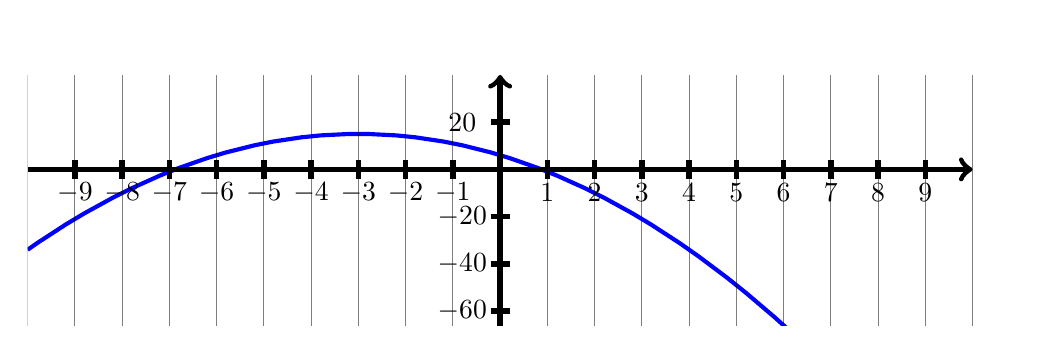
\begin{tikzpicture}[baseline,scale = 0.6]

        \tikzset{
          point/.style={
            thick,
            draw,
            cross out,
            inner sep=0pt,
            minimum width=5pt,
            minimum height=5pt,
          },
        }
        \clip (-10,-3.3) rectangle (11,3);
            
        \draw[color={blue},line width = 1.5] (-10,-1.7)--(-9.8,-1.56)--(-9.6,-1.43)--(-9.4,-1.3)--(-9.2,-1.17)--(-9,-1.05)--(-8.8,-0.93)--(-8.6,-0.82)--(-8.4,-0.71)--(-8.2,-0.6)--(-8,-0.5)--(-7.8,-0.4)--(-7.6,-0.31)--(-7.4,-0.22)--(-7.2,-0.13)--(-7,-0.05)--(-6.8,0.03)--(-6.6,0.1)--(-6.4,0.17)--(-6.2,0.24)--(-6,0.3)--(-5.8,0.36)--(-5.6,0.41)--(-5.4,0.46)--(-5.2,0.51)--(-5,0.55)--(-4.8,0.59)--(-4.6,0.62)--(-4.4,0.65)--(-4.2,0.68)--(-4,0.7)--(-3.8,0.72)--(-3.6,0.73)--(-3.4,0.74)--(-3.2,0.75)--(-3,0.75)--(-2.8,0.75)--(-2.6,0.74)--(-2.4,0.73)--(-2.2,0.72)--(-2,0.7)--(-1.8,0.68)--(-1.6,0.65)--(-1.4,0.62)--(-1.2,0.59)--(-1,0.55)--(-0.8,0.51)--(-0.6,0.46)--(-0.4,0.41)--(-0.2,0.36)--(0,0.3)--(0.2,0.24)--(0.4,0.17)--(0.6,0.1)--(0.8,0.03)--(1,-0.05)--(1.2,-0.13)--(1.4,-0.22)--(1.6,-0.31)--(1.8,-0.4)--(2,-0.5)--(2.2,-0.6)--(2.4,-0.71)--(2.6,-0.82)--(2.8,-0.93)--(3,-1.05)--(3.2,-1.17)--(3.4,-1.3)--(3.6,-1.43)--(3.8,-1.56)--(4,-1.7)--(4.2,-1.84)--(4.4,-1.99)--(4.6,-2.14)--(4.8,-2.29)--(5,-2.45)--(5.2,-2.61)--(5.4,-2.78)--(5.6,-2.95)--(5.8,-3.12)--(6,-3.3)--(6.2,-3.48)--(6.4,-3.67)--(6.6,-3.86)--(6.8,-4.05)--(7,-4.25)--(7.2,-4.45)--(7.4,-4.66)--(7.6,-4.87);
        \draw[color={blue},line width = 1.5] ;
        \draw[color={blue},line width = 1.5] ;
        \draw[color={blue},line width = 1.5] ;
        \draw[color={blue},line width = 1.5] ;
        \draw[color={blue},line width = 1.5] ;
        \draw[color={blue},line width = 1.5] ;
        \draw[color={blue},line width = 1.5] ;
        \draw[color={blue},line width = 1.5] ;
        \draw[color={blue},line width = 1.5] ;
        \draw[color={blue},line width = 1.5] ;
        \draw[color={blue},line width = 1.5] ;
        \draw[color={blue},line width = 1.5] ;
        
        \draw[color ={black},line width = 2,->] (-10,0)--(10,0);
        \draw[color ={black},line width = 2,->] (0,-5)--(0,2);
        \draw[color ={black},opacity = 0.5] (1,-5)--(1,2);
        \draw[color ={black},opacity = 0.5] (2,-5)--(2,2);
        \draw[color ={black},opacity = 0.5] (3,-5)--(3,2);
        \draw[color ={black},opacity = 0.5] (4,-5)--(4,2);
        \draw[color ={black},opacity = 0.5] (5,-5)--(5,2);
        \draw[color ={black},opacity = 0.5] (6,-5)--(6,2);
        \draw[color ={black},opacity = 0.5] (7,-5)--(7,2);
        \draw[color ={black},opacity = 0.5] (8,-5)--(8,2);
        \draw[color ={black},opacity = 0.5] (9,-5)--(9,2);
        \draw[color ={black},opacity = 0.5] (10,-5)--(10,2);
        \draw[color ={black},opacity = 0.5] (-1,-5)--(-1,2);
        \draw[color ={black},opacity = 0.5] (-2,-5)--(-2,2);
        \draw[color ={black},opacity = 0.5] (-3,-5)--(-3,2);
        \draw[color ={black},opacity = 0.5] (-4,-5)--(-4,2);
        \draw[color ={black},opacity = 0.5] (-5,-5)--(-5,2);
        \draw[color ={black},opacity = 0.5] (-6,-5)--(-6,2);
        \draw[color ={black},opacity = 0.5] (-7,-5)--(-7,2);
        \draw[color ={black},opacity = 0.5] (-8,-5)--(-8,2);
        \draw[color ={black},opacity = 0.5] (-9,-5)--(-9,2);
        \draw[color ={black},opacity = 0.5] (-10,-5)--(-10,2);
        \draw[color ={black},line width = 2] (1,-0.2)--(1,0.2);
        \draw[color ={black},line width = 2] (2,-0.2)--(2,0.2);
        \draw[color ={black},line width = 2] (3,-0.2)--(3,0.2);
        \draw[color ={black},line width = 2] (4,-0.2)--(4,0.2);
        \draw[color ={black},line width = 2] (5,-0.2)--(5,0.2);
        \draw[color ={black},line width = 2] (6,-0.2)--(6,0.2);
        \draw[color ={black},line width = 2] (7,-0.2)--(7,0.2);
        \draw[color ={black},line width = 2] (8,-0.2)--(8,0.2);
        \draw[color ={black},line width = 2] (9,-0.2)--(9,0.2);
        \draw[color ={black},line width = 2] (-1,-0.2)--(-1,0.2);
        \draw[color ={black},line width = 2] (-2,-0.2)--(-2,0.2);
        \draw[color ={black},line width = 2] (-3,-0.2)--(-3,0.2);
        \draw[color ={black},line width = 2] (-4,-0.2)--(-4,0.2);
        \draw[color ={black},line width = 2] (-5,-0.2)--(-5,0.2);
        \draw[color ={black},line width = 2] (-6,-0.2)--(-6,0.2);
        \draw[color ={black},line width = 2] (-7,-0.2)--(-7,0.2);
        \draw[color ={black},line width = 2] (-8,-0.2)--(-8,0.2);
        \draw[color ={black},line width = 2] (-9,-0.2)--(-9,0.2);
        \draw[color ={black},line width = 2] (-0.2,1)--(0.2,1);
        \draw[color ={black},line width = 2] (-0.2,-1)--(0.2,-1);
        \draw[color ={black},line width = 2] (-0.2,-2)--(0.2,-2);
        \draw[color ={black},line width = 2] (-0.2,-3)--(0.2,-3);
        \draw[color ={black},line width = 2] (-0.2,-4)--(0.2,-4);
        \draw [color={black},fill opacity = 1] (1,-0.5) node[anchor = center,scale=1] {$1$};
        \draw [color={black},fill opacity = 1] (2,-0.5) node[anchor = center,scale=1] {$2$};
        \draw [color={black},fill opacity = 1] (3,-0.5) node[anchor = center,scale=1] {$3$};
        \draw [color={black},fill opacity = 1] (4,-0.5) node[anchor = center,scale=1] {$4$};
        \draw [color={black},fill opacity = 1] (5,-0.5) node[anchor = center,scale=1] {$5$};
        \draw [color={black},fill opacity = 1] (6,-0.5) node[anchor = center,scale=1] {$6$};
        \draw [color={black},fill opacity = 1] (7,-0.5) node[anchor = center,scale=1] {$7$};
        \draw [color={black},fill opacity = 1] (8,-0.5) node[anchor = center,scale=1] {$8$};
        \draw [color={black},fill opacity = 1] (9,-0.5) node[anchor = center,scale=1] {$9$};
        \draw [color={black},fill opacity = 1] (-1,-0.5) node[anchor = center,scale=1] {$-1$};
        \draw [color={black},fill opacity = 1] (-2,-0.5) node[anchor = center,scale=1] {$-2$};
        \draw [color={black},fill opacity = 1] (-3,-0.5) node[anchor = center,scale=1] {$-3$};
        \draw [color={black},fill opacity = 1] (-4,-0.5) node[anchor = center,scale=1] {$-4$};
        \draw [color={black},fill opacity = 1] (-5,-0.5) node[anchor = center,scale=1] {$-5$};
        \draw [color={black},fill opacity = 1] (-6,-0.5) node[anchor = center,scale=1] {$-6$};
        \draw [color={black},fill opacity = 1] (-7,-0.5) node[anchor = center,scale=1] {$-7$};
        \draw [color={black},fill opacity = 1] (-8,-0.5) node[anchor = center,scale=1] {$-8$};
        \draw [color={black},fill opacity = 1] (-9,-0.5) node[anchor = center,scale=1] {$-9$};
        \draw [color={black},fill opacity = 1] (-0.8,1) node[anchor = center,scale=1] {$20$};
        \draw [color={black},fill opacity = 1] (-0.8,-1) node[anchor = center,scale=1] {$-20$};
        \draw [color={black},fill opacity = 1] (-0.8,-2) node[anchor = center,scale=1] {$-40$};
        \draw [color={black},fill opacity = 1] (-0.8,-3) node[anchor = center,scale=1] {$-60$};
        \draw [color={black},fill opacity = 1] (-0.8,-4) node[anchor = center,scale=1] {$-80$};
    
    \end{tikzpicture}\\
    
\end{exercice}

D'après les coordonnées $(-3;15)$ du sommet, $f$ a pour forme canonique : $f(x)=a(x+3)^2+15$.\\
De plus $f(2)=-10$ donc $a(2+3)^2+15=-10$ soit $25a +15=-10$.\\
On en déduit que $a=\dfrac{-10-15}{25}=-1$.\\
Développons la forme canonique :
\begin{tabbing}
    $f(x)$  \= $ =-(x+3)^2+15$\\
    \>  $=-(x^2{\color{green}\boldsymbol{+6}}x+{\color{red}\boldsymbol{9}}){\color{red}\boldsymbol{+15}}$\\
    \>  $={\color{blue}\boldsymbol{-}}x^2{\color{green}\boldsymbol{-6}}x{\color{red}\boldsymbol{+6}}$
\end{tabbing} 
  


\end{document}